% !TEX program = xelatex
\documentclass[11pt,letterpaper]{article}
\usepackage{fontspec}
\usepackage[spanish,es-nodecimaldot]{babel}
\usepackage[margin=2.2cm]{geometry}
\usepackage{graphicx,float,booktabs,tabularx,longtable,array,enumitem,amssymb}
\usepackage[hidelinks]{hyperref}
\usepackage{xcolor,fancyhdr}
\usepackage{tikz}
\usetikzlibrary{arrows.meta,positioning,fit}
\graphicspath{{../../../artifacts/entrega2/figuras/}}
\setlength{\parskip}{4pt}\setlength{\parindent}{0pt}
\pagestyle{fancy}\fancyhf{}
\fancyhead[L]{MINE-4214 · Proyecto Entrega 2}\fancyhead[R]{CupiTaller · Universidad de los Andes}
\fancyfoot[C]{\thepage}
\setcounter{secnumdepth}{2}
\newcolumntype{L}{>{\raggedright\arraybackslash}X}
\newcolumntype{R}{>{\raggedleft\arraybackslash}r}
\newcommand{\pendiente}[1]{\textcolor{red}{\textbf{[TODO: #1]}}}
\newcommand{\cod}[1]{\texttt{\small #1}}
\tikzset{
  caja/.style={draw=black!45, rounded corners=2pt, align=center, font=\footnotesize, inner sep=4pt, minimum height=0.95cm, text width=2.1cm, fill=white, execute at begin node={\hyphenpenalty=10000 \exhyphenpenalty=10000 }},
  dato/.style={caja, fill=black!6},
  modelo/.style={caja, fill=blue!8, draw=blue!45},
  flecha/.style={-{Stealth[length=5pt]}, draw=black!60, line width=0.5pt},
  nota/.style={font=\scriptsize, text=black!65, align=center},
}
\begin{document}
\begin{center}
{\Large\bfseries Proyecto · Entrega 2\\[2pt] Documentos del curso y bodega de CupiTaller:\\ prompting directo, RAG y agente híbrido}\\[8pt]
MINE-4214 Modelado y Diseño de Datos\\
Universidad de los Andes · Noviembre de 2026\\[6pt]
\textbf{Integrantes:} \emph{María Alejandra Pérez Petro}, \emph{Santiago Martinez Novoa}
\end{center}

\textbf{Resumen.} CupiTaller es el centro de tutorías del curso Introducción a la Programación (IP). Su conocimiento cualitativo está en 58 documentos (dos versiones del programa del curso y 56 presentaciones de clase) y su operación en la bodega de la Entrega 1 (83.894 reservas y 60.024 encuestas, de 2016-20 a 2026-10). Implementamos dos formas de responder con los documentos y las medimos con 26 preguntas: el prompting directo acertó 26, un RAG sobre transcripciones con visión 23 y un RAG sobre la capa de texto de los PDF 18, porque el código de las presentaciones está en capturas de pantalla. El prompting directo cuesta entre 7 y 71 veces más por consulta que el RAG y ocupa el 10\,\% de la ventana de contexto con un solo semestre de documentos. Cuando el corpus mezcla el programa de 2020-20 con el vigente, un RAG sin etiquetas responde con la regla antigua en 3 de 6 preguntas; un filtro de vigencia lo corrige. Un agente que consulta el RAG y ejecuta SQL sobre la bodega muestra, por ejemplo, que las tutorías grupales que anuncia el programa de 2020-20 no registran reservas desde 2021-20.

\tableofcontents
\bigskip

\section{Fase 1 · Requerimientos analíticos}

\subsection{Dominio de negocio}

El dominio es la \textbf{gestión del servicio de tutorías de CupiTaller}, del Departamento de Ingeniería de Sistemas y Computación de la Universidad de los Andes. En CupiTaller, monitores atienden con cita previa a estudiantes de IP y de otros cursos de programación. La Entrega 1 modeló la operación del servicio: reservas, estados, encuestas previas y de satisfacción, exportadas de la plataforma Bookeau.

La operación responde a reglas que no están en Bookeau. Están en documentos: el \textbf{programa del curso} fija qué puede y qué no puede hacer un tutor, cómo se evalúa cada nivel y qué contenido puede usar un estudiante; las \textbf{presentaciones de clase} definen qué se ha enseñado hasta cada nivel. Esta entrega une las dos fuentes.

\subsection{Requerimiento 1 · Contenido por nivel y su evolución (solo documentos)}

\begin{table}[H]\small\renewcommand{\arraystretch}{1.2}
\begin{tabularx}{\textwidth}{>{\raggedright\arraybackslash}p{0.2\textwidth}L}
\toprule
\textbf{Elemento} & \textbf{Definición} \\
\midrule
Decisión que apoya & Qué puede explicar un tutor en una tutoría y con qué ejemplos. El programa exige que el estudiante use «únicamente el contenido autorizado, es decir, los temas y la sintaxis estudiados hasta el nivel del curso», y prohíbe a los tutores solucionar tareas, quices o proyectos. Un tutor que resuelve una duda de Nivel 2 con un ciclo \cod{for}, que se enseña en Nivel 3, pone al estudiante en riesgo de una sanción. \\
Rol beneficiado & \textbf{Monitores de CupiTaller}, durante la tutoría, y la \textbf{coordinación académica}, que los forma cada semestre. Los monitores cambian cada semestre y muchos cursaron IP con otra versión del material. También los \textbf{profesores} de IP, que preparan su nivel y necesitan saber qué se dicta hoy que no estaba en el material de semestres anteriores. \\
Preguntas & ¿En qué nivel se introduce un tema? ¿Cómo lo explica el curso y con qué ejemplo de código? ¿Un estudiante de Nivel 2 ya vio ciclos? ¿Qué convenciones de estilo exige el curso? ¿Qué se dicta hoy en un nivel que no estaba en versiones anteriores del curso? \\
Fuentes & El programa vigente y las 44 presentaciones vigentes; para comparar versiones, las 12 presentaciones de 2020-20 y 2021-10. No requiere la bodega. \\
\bottomrule
\end{tabularx}
\end{table}

\subsection{Requerimiento 2 · Vigencia y cumplimiento de las reglas del servicio (documentos y bodega)}

\begin{table}[H]\small\renewcommand{\arraystretch}{1.2}
\begin{tabularx}{\textwidth}{>{\raggedright\arraybackslash}p{0.2\textwidth}L}
\toprule
\textbf{Elemento} & \textbf{Definición} \\
\midrule
Decisión que apoya & Qué reglas del servicio hay que actualizar en los documentos, dónde reforzar la oferta de tutores y qué reforzar en su formación. La coordinación necesita saber si lo que los documentos prometen coincide con lo que ocurre. \\
Rol beneficiado & \textbf{Coordinación de CupiTaller}, la misma destinataria del Análisis 1 de la Entrega 1: planea las franjas, asigna monitores y fija las reglas de reserva. \\
Preguntas & ¿Se siguen ofreciendo los tipos de tutoría que anuncia el programa? ¿A qué dedican los estudiantes la tutoría, frente a lo que el programa permite al tutor? ¿La demanda sigue la estructura de niveles que define el programa? ¿Qué reportan las encuestas sobre el uso de IA por los tutores? \\
Por qué no basta una sola fuente & El documento dice qué debería pasar y la bodega qué pasó. Ninguna de las dos responde sola si una regla se cumple o si un documento quedó desactualizado. \\
\bottomrule
\end{tabularx}
\end{table}

\subsection{Fuentes no estructuradas}

El corpus tiene \textbf{58 documentos y 716 páginas}. Los documentos vigentes los entrega la coordinación del curso para 2026-20; los históricos son de los periodos de 2020-20 y 2021-10.

\begin{table}[H]\small\renewcommand{\arraystretch}{1.15}
\begin{tabularx}{\textwidth}{L>{\raggedright\arraybackslash}p{0.13\textwidth}RRL}
\toprule
\textbf{Documento} & \textbf{Semestre} & \textbf{Archivos} & \textbf{Páginas} & \textbf{Conocimiento que aporta} \\
\midrule
Programa del curso IP & 2026-20 & 1 & 6 & Niveles, evaluación, integridad académica y reglas de CupiTaller vigentes \\
Presentaciones de clase, niveles 1 a 4 & 2026-20 & 44 & 571 & Temas, sintaxis y ejemplos de código por nivel (11, 11, 12 y 10 presentaciones) \\
Programa del curso IP & 2020-20 & 1 & 6 & Versión anterior de las mismas reglas; es un PDF escaneado, sin capa de texto \\
Presentaciones de clase de una sección & 2020-20 y 2021-10 & 12 & 133 & Versión anterior del material de los cuatro niveles \\
\bottomrule
\end{tabularx}
\end{table}

Cada documento se etiqueta en un catálogo (\cod{data/plata/documentos/catalogo\_documentos.csv}) con su semestre, si está vigente, su nivel y su tipo. El catálogo se propone a partir del nombre del archivo, de su fecha de creación y de la portada, y se corrige a mano. Las portadas de las presentaciones históricas llevan el nombre y el correo de quien dictó la sección; por eso se omiten y no se indexan ni se envían al modelo.

\subsection{Fuentes estructuradas: indicadores de la bodega}

El Requerimiento 2 usa la bodega Gold de la Entrega 1 (modelo dimensional de Kimball en SQLite), reconstruida con las reglas R01 a R07: \textbf{83.894 reservas de tutoría}, 60.024 encuestas y sus respuestas. Los indicadores son los de la Entrega 1, incluida la oferta de cupos, y dos nuevos que salen de las mismas tablas de hechos.

\begin{table}[H]\small\renewcommand{\arraystretch}{1.15}
\begin{tabularx}{\textwidth}{>{\raggedright\arraybackslash}p{0.27\textwidth}L>{\raggedright\arraybackslash}p{0.2\textwidth}}
\toprule
\textbf{Indicador} & \textbf{Definición} & \textbf{Origen} \\
\midrule
Reservas por período y por semana & Conteo de reservas de tutoría & \cod{hecho\_reserva} (Entrega 1) \\
Tasa de inasistencia & No asistió / (Atendida + No asistió) & \cod{hecho\_reserva}, Análisis 1 \\
Proporción en cola & En cola / reservas & \cod{hecho\_reserva}, Análisis 1 \\
Calificación del tutor & Media y proporción de calificaciones 1 a 3 & \cod{hecho\_encuesta}, Análisis 2 \\
Uso declarado de la tutoría & Distribución de la respuesta «La mayor parte del tiempo de la tutoría lo dediqué a» & \cod{hecho\_respuesta} (nuevo) \\
Tipos de horario por período & Reservas por tipo de horario, incluidos los descontinuados & Silver de la Entrega 1 (nuevo) \\
Capacidad y ocupación & Cupos disponibles y cupos reservados / cupos disponibles, por franja (período, día y hora) y por semestre, categoría Tutor Presencial & \cod{hecho\_oferta} (Entrega 1) \\
Lista de espera por franja & Por período, día y hora: solicitudes en cola, cola que terminó en reserva, asistencias e inasistencias & \cod{hecho\_oferta} (Entrega 1) \\
\bottomrule
\end{tabularx}
\end{table}

El indicador de tipos de horario exigió una tabla agregada nueva, \cod{agg\_tipos\_de\_horario}. La regla R03 de la Entrega 1 deja en Gold solo los tipos Normal, Express y Normal pico, y los tipos descontinuados son justo la evidencia que necesita este requerimiento. La tabla cuenta en Silver las 86.562 reservas por período, tipo de horario y estado, sin datos personales.

La oferta es la tabla de hechos \cod{hecho\_oferta} de la Entrega 1: 1.396 franjas (período, día y hora) con su capacidad, sus cupos reservados y los cinco conteos de lo ocurrido, cargadas de los 30 reportes de horarios de Bookeau. La bodega le suma \cod{agg\_oferta\_periodo}, con la capacidad, la ocupación y la cobertura de los 19 semestres de la tabla de oferta de la Entrega 1. Al construirla se comprueba que la capacidad por franja sume la de cada semestre, y suma igual en los 19. Las cifras de la Entrega 1 se reproducen: ocupación total de 74,5\,\% y 1.001 franjas con lista de espera.

\subsection{El cruce}

La unión de las dos fuentes produce hallazgos que ninguna da sola. Cuatro ejemplos, desarrollados en la sección~\ref{sec:agente}:

\begin{itemize}[leftmargin=1.5em,itemsep=2pt]
\item El programa de 2020-20 anuncia tutorías «individuales, grupales y express». La bodega registra la última reserva grupal en 2021-20. El documento está desactualizado, y un asistente que lo cite informa mal al estudiante.
\item El programa vigente dice que los tutores «no solucionan una tarea, quiz o proyecto». En las encuestas, el 52\,\% de los estudiantes dice que dedicó la mayor parte de la tutoría a «resolver un problema en mi proyecto» (10.236 de 19.672 respuestas). La regla y el uso real del servicio están en tensión, y la coordinación debe decidir cómo formar a los tutores para ese caso.
\item El programa organiza el curso en cuatro niveles, cada uno con un proyecto y un examen. Las reservas de IP llegan en cuatro olas por semestre que caen después de cada pico. La oferta de tutores se puede planear con el calendario de niveles.
\item La capacidad no siguió a la demanda: 2.616 cupos tanto en 2025-20 como en 2026-10, con ocupación de 54 y 55\,\%. En 2026-10 la lista de espera se concentra en los miércoles: a las 14:00 hubo 8 solicitudes con 44 de 55 cupos reservados. Ningún documento del corpus fija una regla de cupos, así que la decisión de reasignarlos es de la coordinación y estos datos le dicen dónde.
\end{itemize}

\section{Fase 2 · Prompting directo frente a RAG}

\subsection{Los dos enfoques implementados}

\begin{figure}[H]\centering
\begin{tikzpicture}[node distance=0.45cm and 0.36cm]
\node[dato] (docs) {58 documentos\\PDF y PPTX};
\node[caja, right=of docs] (cat) {Catálogo:\\semestre, vigencia, nivel};
\node[caja, right=of cat] (png) {Página\\como imagen};
\node[modelo, right=of png] (ocr) {Transcripción con visión\\(gpt-6-luna)};
\node[caja, right=of ocr] (emb) {Chunk por página\\y embedding (e5-small)};
\node[dato, right=of emb] (pg) {pgvector:\\colecciones texto y visual};
\draw[flecha] (docs)--(cat); \draw[flecha] (cat)--(png); \draw[flecha] (png)--(ocr); \draw[flecha] (ocr)--(emb); \draw[flecha] (emb)--(pg);
\node[nota, anchor=south west] at ([yshift=0.08cm]docs.north west) {\textbf{Ingesta}, una vez por documento};

\node[caja, below=1.75cm of docs] (q) {Pregunta};
\node[caja, below=1.55cm of ocr] (full) {Todos los documentos transcritos\\(103.160 tokens)};
\node[modelo, below=1.75cm of emb] (llm1) {gpt-6-luna};
\node[caja, below=1.75cm of pg] (a1) {Respuesta\\con citas};
\draw[flecha] (q.east)--(q.east -| full.west); \draw[flecha] (llm1.west -| full.east)--(llm1.west); \draw[flecha] (llm1)--(a1);
\draw[flecha, dashed] (ocr.south) -- (full.north);
\node[nota, anchor=south west] at ([yshift=0.08cm]q.north west) {\textbf{Enfoque 1}, prompting directo};

\node[caja, below=1.75cm of q] (q2) {Pregunta};
\node[caja, below=1.35cm of full] (top) {5 fragmentos más parecidos\\(filtro de vigencia)};
\node[modelo, below=1.75cm of llm1] (llm2) {gpt-6-luna};
\node[caja, below=1.75cm of a1] (a2) {Respuesta\\con citas};
\draw[flecha] (q2.east)--(q2.east -| top.west); \draw[flecha] (llm2.west -| top.east)--(llm2.west); \draw[flecha] (llm2)--(a2);
\draw[flecha, dashed] (pg.east) -- ++(0.3,0) |- ([yshift=-0.45cm]top.south) -- (top.south);
\node[nota, anchor=south west] at ([yshift=0.08cm]q2.north west) {\textbf{Enfoque 2}, RAG};
\end{tikzpicture}
\caption{Ingesta y los dos enfoques. Ambos responden con el mismo modelo y las mismas reglas de respuesta; solo cambia el contexto que recibe el modelo.}
\label{fig:arquitectura}
\end{figure}

\textbf{Enfoque 1, prompting directo} (\cod{src/entrega2/enfoques.py}, \cod{responder\_directo}). El prompt lleva los 45 documentos vigentes completos, página por página, cada uno con un encabezado que indica título, nivel, semestre y vigencia. Son 52.607 palabras y 103.160 tokens por consulta. Los documentos van antes de la pregunta y terminan en un punto de corte de caché, para que las consultas siguientes lean ese prefijo de la caché del proveedor.

\textbf{Enfoque 2, RAG} (\cod{src/entrega2/indexar.py}, \cod{src/entrega2/base\_vectorial.py}, \cod{responder\_rag}). La base vectorial es Postgres 18 con pgvector, con el esquema del laboratorio del curso y dos cambios: el semestre, la vigencia y el nivel son columnas del documento, y cada fragmento pertenece a una colección. La unidad de chunking es la página, porque una diapositiva desarrolla una idea; solo se parten las páginas de más de 200 palabras, entre líneas para no romper el código. Los embeddings son de \cod{multilingual-e5-small} (384 dimensiones, se ejecuta en local) y la búsqueda usa distancia coseno sobre un índice HNSW. La consulta recupera los 5 fragmentos más parecidos y el modelo responde solo con ellos.

Los dos enfoques usan \cod{gpt-6-luna} sin razonamiento, como el laboratorio del curso, y las mismas instrucciones: responder solo con las fuentes, citar, y decir «No hay información suficiente en las fuentes» cuando no alcancen.

\subsection{Ingesta: por qué hace falta visión}

Las presentaciones vigentes llevan el código como capturas de pantalla, y el programa de 2020-20 es un escaneo. La capa de texto de los PDF vigentes tiene 23.203 palabras; la transcripción con visión de las mismas páginas tiene 49.673 (figura~\ref{fig:palabras}). El Nivel 4, el más visual, pasa de 3.101 a 11.132 palabras.

\begin{figure}[H]\centering
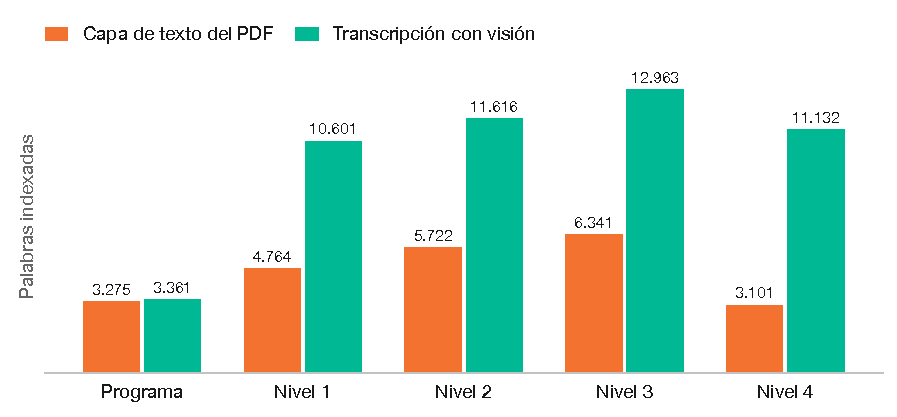
\includegraphics[width=0.86\textwidth]{palabras_por_ingesta.pdf}
\caption{Palabras indexadas de los documentos vigentes con cada forma de ingesta.}
\label{fig:palabras}
\end{figure}

Usamos la visión al ingerir y no al buscar. Cada página se renderiza como imagen y el modelo la transcribe una vez a Markdown: texto, código de las capturas con su indentación, tablas y una línea por figura (\cod{src/entrega2/transcribir.py}). El resultado se indexa con embeddings de texto. La alternativa, embeddings visuales de página (del tipo ColPali), exige varios vectores por página y otro modelo, y no cabe en el esquema de un vector por fragmento de la base del curso. Transcribir las 716 páginas tomó 716 llamadas (mediana de 1,9 s por página), 1,48 millones de tokens de entrada y 122 mil de salida: \textbf{US\$\,0,21} a precio de lista. Los embeddings y la carga de las dos colecciones tomaron 17 s en un portátil.

Para medir el efecto de la ingesta hay dos colecciones sobre los mismos documentos: \cod{texto} (capa de texto del PDF, 732 fragmentos) y \cod{visual} (transcripciones, 753 fragmentos).

\subsection{Evaluación}

Un banco de \textbf{26 preguntas} con respuesta esperada y página de origen (\cod{data/bronce/evaluacion/preguntas.json}) cubre cinco tipos: 7 sobre el programa, 5 sobre contenido que está en el texto de una diapositiva, 6 sobre contenido que solo está en una imagen, 4 sobre el nivel en que se enseña un tema y 4 que el corpus no responde. Tres sistemas responden cada pregunta una vez con los documentos vigentes: prompting directo, RAG de texto y RAG visual.

Un modelo distinto del generador, \cod{gpt-6-sol}, califica cada respuesta contra la esperada como correcta, parcial o incorrecta, y marca si afirma un hecho que contradice lo esperado (\cod{src/entrega2/juez.py}). Revisamos a mano todos los veredictos distintos de «correcta». Una primera corrida mostró que cuatro respuestas esperadas pedían más de lo que preguntaba la pregunta; las ajustamos y volvimos a responder y a calificar todo.

\subsection{Resultados}

\begin{table}[H]\small\renewcommand{\arraystretch}{1.15}\centering
\begin{tabular}{lrrr}
\toprule
\textbf{Medida} & \textbf{Prompting directo} & \textbf{RAG de texto} & \textbf{RAG visual} \\
\midrule
Respuestas correctas (de 26) & 26 & 18 & 23 \\
Parciales / incorrectas & 0 / 0 & 2 / 6 & 1 / 2 \\
Respuestas con un hecho inventado & 0 & 0 & 0 \\
Página esperada entre los 5 fragmentos (de 22) & no aplica & 21 & 21 \\
Tokens de entrada por consulta & 103.160 & 1.109 & 1.255 \\
Tokens de salida por consulta & 48 & 33 & 38 \\
Latencia mediana (s) & 1,44 & 1,08 & 1,12 \\
Costo por 1.000 consultas, sin caché (USD) & 10,34 & 0,13 & 0,14 \\
Costo por 1.000 consultas, caché caliente (USD) & 1,06 & 0,13 & 0,14 \\
\bottomrule
\end{tabular}
\caption{Resultados sobre las 26 preguntas. Precio de lista de \cod{gpt-6-luna}: US\$\,0,10 por millón de tokens de entrada, 0,01 leídos de caché y 0,50 de salida.}
\label{tab:resultados}
\end{table}

\begin{figure}[H]\centering
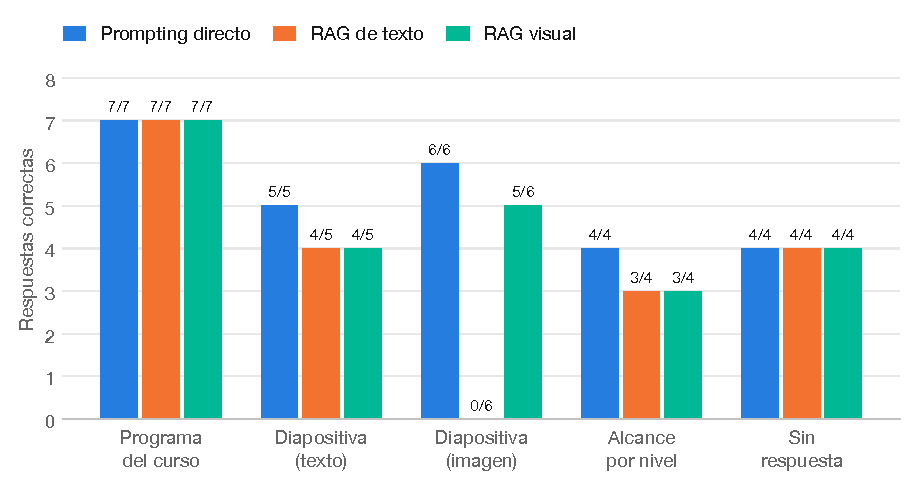
\includegraphics[width=0.88\textwidth]{exactitud_por_categoria.pdf}
\caption{Respuestas correctas por tipo de pregunta.}
\label{fig:exactitud}
\end{figure}

\textbf{La ingesta pesa más que el enfoque.} El RAG de texto no acertó ninguna de las 6 preguntas cuyo contenido está en una imagen; el RAG visual acertó 5. En las dos colecciones la página esperada estuvo entre los 5 fragmentos en 21 de 22 preguntas: el RAG de texto encuentra la página correcta, pero el fragmento no contiene el código. En sus seis respuestas incorrectas dijo que no había información suficiente.

\textbf{El prompting directo acertó las 26.} Con todo el corpus a la vista responde las dos preguntas que el RAG visual no pudo. La primera pide las librerías que presenta la introducción a librerías del Nivel 4: cada librería está en una diapositiva distinta, casi sin texto, y los 5 fragmentos no las reúnen. La segunda pregunta si un estudiante de Nivel 2 ya vio ciclos: el RAG recuperó las diapositivas de \cod{while} y \cod{for}, pero con 5 fragmentos no puede afirmar que algo \emph{no} se enseña antes.

\textbf{Ningún sistema inventó.} Los tres se abstuvieron en las 4 preguntas sin respuesta en el corpus, y ningún veredicto marcó un hecho inventado. El RAG falla por omisión: se abstiene cuando la evidencia no llegó al contexto.

\begin{figure}[H]\centering
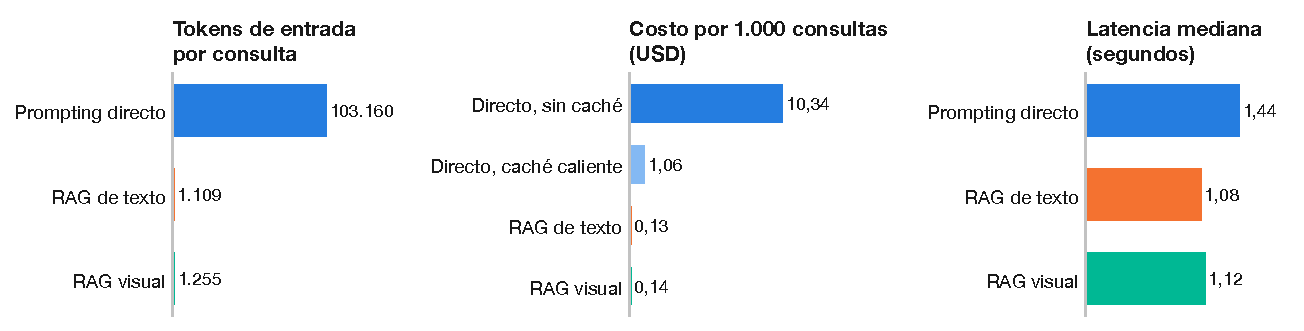
\includegraphics[width=\textwidth]{costo_y_latencia.pdf}
\caption{Tokens, costo y latencia por consulta.}
\label{fig:costo}
\end{figure}

\textbf{El costo del prompting directo depende de la caché.} Sin caché, cada consulta paga los 103.160 tokens: US\$\,0,0103, 71 veces el RAG visual. La caché del proveedor no se activó sola: en el modo por defecto el punto de corte queda al final del mensaje, después de la pregunta, y como la pregunta cambia en cada llamada el prefijo nunca se reutiliza (1 lectura de caché en 35 llamadas). Con un punto de corte explícito al final de los documentos, la primera consulta paga la escritura (US\$\,0,0129) y las siguientes, durante 30 minutos, leen el prefijo a una décima del precio: US\$\,0,0011, 7 veces el RAG visual.

\textbf{La latencia es parecida.} La mediana fue 1,44 s para el prompting directo con caché (1,9 s sin caché) y 1,1 s para el RAG. La búsqueda vectorial tomó 0,03 s; casi todo el tiempo es la generación.

\textbf{Límites de la medición.} Son 26 preguntas y una sola corrida por sistema: una pregunta equivale a 3,8 puntos porcentuales, y en la primera corrida el prompting directo se abstuvo en la pregunta de las librerías, que en la segunda acertó. Las preguntas las escribió el equipo conociendo el corpus. Los precios vienen de rastreadores de precios que citan la página oficial de OpenAI, consultados el 24 de noviembre de 2026.

\subsection{Matriz comparativa}

\begin{table}[H]\footnotesize\renewcommand{\arraystretch}{1.2}
\begin{tabularx}{\textwidth}{>{\raggedright\arraybackslash}p{0.2\textwidth}LL}
\toprule
\textbf{Criterio y definición} & \textbf{Enfoque 1 · Prompting directo} & \textbf{Enfoque 2 · RAG} \\
\midrule
\textbf{Costo de inferencia.} Dólares por consulta, según los tokens de entrada y de salida. & US\$\,10,34 por 1.000 consultas sin caché y 1,06 con caché caliente. El costo crece con el tamaño del corpus. & US\$\,0,14 por 1.000 consultas. No depende del tamaño del corpus. Los embeddings se calculan en local, sin costo por consulta. \\
\textbf{Latencia.} Segundos entre la pregunta y la respuesta completa. & Mediana de 1,44 s con caché y 1,9 s sin ella. & Mediana de 1,1 s; la búsqueda aporta 0,03 s. \\
\textbf{Riesgo de alucinación.} Probabilidad de afirmar algo que las fuentes no dicen o que ya no aplica. & Ningún hecho inventado en 26 respuestas. Si recibe dos versiones de un documento, las ve juntas y puede distinguirlas (sección~\ref{sec:poc}). & Ningún hecho inventado en 52 respuestas. Falla por omisión: se abstiene si la evidencia no llega. Sin etiquetas de vigencia responde con reglas antiguas (3 de 6 preguntas, sección~\ref{sec:poc}). \\
\textbf{Límite de tokens.} Cuánto del contexto del modelo ocupa la consulta. & 103.160 tokens, el 10\,\% de la ventana de \cod{gpt-6-luna} (cerca de 1,05 millones), con un solo semestre de un solo curso. El corpus completo de 58 documentos ya son 65.289 palabras. Unas diez versiones semestrales agotan la ventana. & 1.255 tokens por consulta, constantes aunque el corpus crezca. \\
\textbf{Mantenimiento de la base de conocimiento.} Trabajo para incorporar, cambiar o retirar un documento. & Basta cambiar el archivo y su transcripción. No hay índice ni servidor. Cualquier cambio invalida la caché. & Hay que transcribir, calcular embeddings y recargar el documento, mantener el catálogo de vigencia y operar Postgres. El paso es automático (\cod{src/entrega2/main.py}) y solo reprocesa lo que cambió. \\
\textbf{Cobertura del contenido visual} (criterio añadido). Si el sistema ve lo que está en imágenes. & Depende de la ingesta, no del enfoque: con la capa de texto del PDF perdería el código de las capturas. & Igual. Con la capa de texto acertó 0 de 6 preguntas de contenido en imagen; con la transcripción, 5 de 6. \\
\textbf{Preguntas sobre el conjunto} (criterio añadido). Preguntas que piden reunir varias páginas o afirmar una ausencia. & Las responde: ve todo el corpus (4 de 4 de alcance por nivel). & Limitado por los k fragmentos (3 de 4). \\
\textbf{Control por metadatos} (criterio añadido). Restringir la respuesta por vigencia, nivel o tipo de documento. & Solo eligiendo qué archivos entran al prompt. & Un filtro SQL sobre las columnas del documento, por consulta. \\
\bottomrule
\end{tabularx}
\end{table}

\subsection{Lineamientos corporativos}

\textbf{Usar prompting directo cuando} se cumplen estas condiciones: el material cabe con holgura en la ventana (como regla, menos de una quinta parte); son pocos documentos de una sola versión, o justamente se quieren comparar dos versiones; la pregunta pide una visión de conjunto; y el uso es ocasional. Ejemplos en CupiTaller: comparar el programa de este semestre con el anterior antes de publicarlo, o resumir qué cambió en un nivel. No requiere infraestructura. Marcar siempre el punto de corte de caché después de los documentos.

\textbf{Invertir en RAG cuando} se cumple alguna de estas: el corpus crece cada semestre o reúne varios cursos y versiones; el volumen de consultas es alto o continuo; hace falta restringir por vigencia, nivel o curso; hay que mostrar la página que sustenta la respuesta; o los documentos serán una herramienta de un agente. Un RAG exige dos cosas que el prompting directo perdona: una ingesta que capture el contenido visual y un catálogo de vigencia mantenido por alguien.

\textbf{En ambos casos:} no enviar datos personales a un modelo externo, citar documento, semestre y página, y permitir la abstención.

\subsection{Selección y justificación para el Requerimiento 1}

Para el Requerimiento 1 (contenido autorizado por nivel, para monitores) recomendamos el \textbf{RAG visual con filtro de vigencia}, y reservamos el prompting directo para consultas de conjunto acotadas a un nivel.

\textbf{Escalabilidad.} Hoy el prompting directo es el más exacto (26 de 26 frente a 23) porque el corpus de un semestre cabe en la ventana. No se sostiene: CupiTaller atiende también EDA e IP Honores, y conservar las versiones anteriores para saber con qué material cursó cada monitor multiplica el corpus por el número de semestres. Cada versión semestral de IP añade unos 100.000 tokens al prompt de \emph{todas} las consultas; el RAG mantiene 1.255 tokens por consulta y solo crece el índice.

\textbf{Costo-beneficio.} A la escala actual el costo no decide: 10.000 consultas por semestre cuestan US\$\,1,45 con RAG y entre US\$\,10,6 y 103 con prompting directo, según la caché. La transcripción, el paso más costoso, es común a los dos enfoques (US\$\,0,21 por todo el corpus). Deciden tres capacidades que solo tiene el RAG: filtrar por vigencia, sin lo cual el sistema responde con reglas antiguas; devolver la diapositiva exacta que el monitor puede mostrar al estudiante; y servir de herramienta al agente del Requerimiento 2. El costo del RAG es operativo: una base Postgres y un catálogo que alguien mantiene.

\textbf{Lo que se pierde y cómo se compensa.} El RAG falló dos preguntas de conjunto. Para ese tipo de pregunta, el prompting directo con las presentaciones de un solo nivel (cerca de una cuarta parte del corpus) da la visión completa a una fracción del costo.

\section{Fase 3 · Retos documentales e integración híbrida}

\subsection{El reto: dos versiones del programa que se contradicen}

El programa del curso existe en al menos dos versiones que circulan entre monitores y estudiantes. La de 2020-20 se escribió para clases virtuales; la de 2026-20 cambió la evaluación, la integridad académica y la descripción de CupiTaller.

\begin{table}[H]\small\renewcommand{\arraystretch}{1.15}
\begin{tabularx}{\textwidth}{>{\raggedright\arraybackslash}p{0.22\textwidth}LL}
\toprule
\textbf{Regla} & \textbf{Programa 2020-20} & \textbf{Programa 2026-20 (vigente)} \\
\midrule
Peso de los niveles 1 a 4 & 10, 25, 35 y 30\,\% & 10, 20, 35 y 35\,\% \\
Proyecto de cada nivel & Tiene nota (4 a 6\,\%) y se anula si el examen queda bajo el 60\,\% de la nota del proyecto & No tiene nota; los monitores dan retroalimentación formativa \\
Proyecto que no es de autoría propia & Cláusula de arrepentimiento: avisar en 72 horas deja en cero el proyecto, no el nivel & Sin cláusula; nota de cero o remisión al Comité Disciplinario \\
Tipos de tutoría en CupiTaller & Individuales, grupales y express & Tutorías personalizadas con reserva; no enumera tipos \\
Plataforma del curso & Brightspace & Bloque Neón \\
Ejercicios en Senecode & Más de 100 & Más de 200, en cuatro dificultades \\
\bottomrule
\end{tabularx}
\end{table}

El corpus tiene otras tres fuentes de inconsistencia. Los archivos no dicen su versión: las presentaciones históricas se llaman «C11 - Listas - Copy.pdf» y su semestre solo se infiere de la fecha de creación del archivo. Hay material de curso y material de sección: las presentaciones históricas son de una sección, con su propio orden, y conviven con las oficiales. Y los documentos remiten a otros que no están en el corpus, como el cronograma y los términos de uso de CupiTaller.

\subsection{Prueba de concepto: el RAG recupera la regla desactualizada}
\label{sec:poc}

Seis preguntas cuya respuesta cambió entre las dos versiones (\cod{data/bronce/evaluacion/preguntas\_vigencia.json}) se respondieron con cinco configuraciones (\cod{src/entrega2/poc\_entropia.py}). El «RAG ingenuo» indexa los 58 documentos sin usar ninguna etiqueta del catálogo, como queda un RAG al indexar una carpeta de PDF.

\begin{figure}[H]\centering
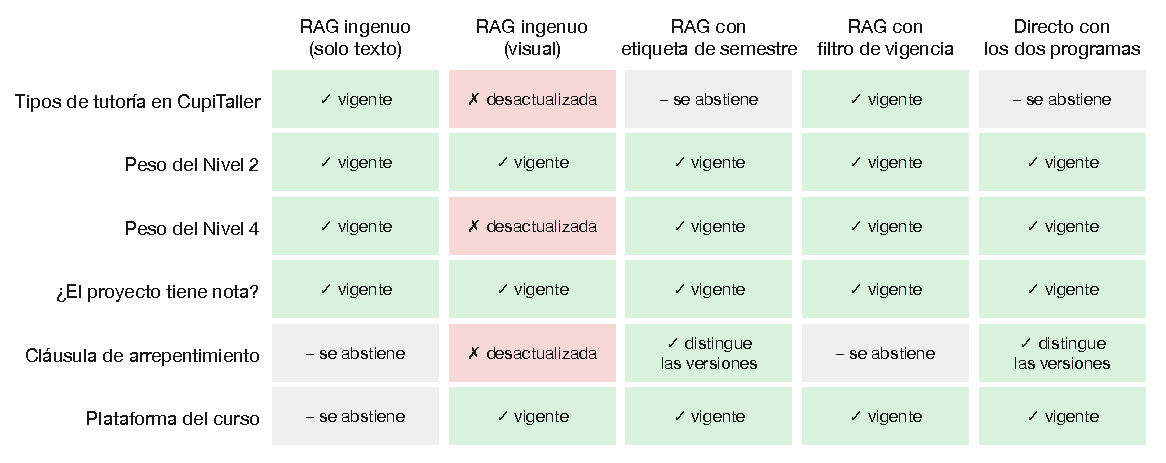
\includegraphics[width=\textwidth]{entropia_poc.pdf}
\caption{Con qué versión coincide la respuesta de cada configuración.}
\label{fig:entropia}
\end{figure}

\textbf{El RAG ingenuo sobre las transcripciones respondió con la regla antigua en 3 de 6 preguntas}, sin advertir que venía de otra versión:

\begin{itemize}[leftmargin=1.5em,itemsep=2pt]
\item «¿Qué tipos de tutorías ofrece CupiTaller?» Respuesta: «CupiTaller ofrece tutorías individuales, grupales y express. [1]». El fragmento más parecido era la página 5 del programa de 2020-20, que enumera los tipos; el programa vigente no los enumera y quedó en segundo lugar.
\item «¿Cuánto vale el Nivel 4 en la nota del curso?» Respuesta: «El Nivel 4 vale el 30\,\% de la nota del curso. [3]». Entre los 5 fragmentos estaban las tablas de ambas versiones y el modelo eligió la antigua.
\item «Si entrego un proyecto que no es de mi autoría pero lo informo en 72 horas, ¿qué pasa?» Respuesta: «La nota del proyecto será cero, pero no la nota completa del nivel. No habrá acción disciplinaria adicional». Esa cláusula ya no existe. Un estudiante que actúe según esta respuesta se expone a un proceso disciplinario.
\end{itemize}

\textbf{El RAG ingenuo de solo texto no dio ninguna respuesta antigua}, y no por diseño: el programa de 2020-20 es un escaneo sin capa de texto y ese RAG no lo ve. Mejorar la ingesta hizo visible el documento antiguo y, con él, el problema. Una ingesta mejor necesita un control de vigencia mejor.

\textbf{Las tres mitigaciones eliminaron las respuestas antiguas.} Con el filtro de vigencia, el RAG solo busca en documentos vigentes: 5 respuestas vigentes y 1 abstención (sobre la cláusula que ya no existe, donde abstenerse es correcto). Con la etiqueta de semestre en cada fuente, el modelo ve ambas versiones y, en el caso de la cláusula, explicó que la versión anterior la tenía y la vigente no. El prompting directo con los dos programas se comportó igual. La etiqueta informa más; el filtro es más seguro para un asistente de estudiantes.

\subsection{Versiones del curso por nivel}
\label{sec:versiones}

La tabla de temas del programa es la misma en 2020-20 y en 2026-20: cuatro niveles de 9, 12, 15 y 12 sesiones, con el mismo tema cada uno. El programa cambió en la evaluación y en las reglas (cuadro anterior); los cambios de temas están en las presentaciones. Eso necesita saberlo un profesor que prepara su nivel con material de semestres anteriores, y un monitor que decide qué puede explicar.

Para medirlo, cada presentación de 2026-20 se comparó con las 12 presentaciones de 2020-20 y 2021-10 (\cod{src/auxiliar/e2\_temas\_por\_nivel.py}). Una clase tiene versión anterior si el tema principal de su título aparece como sección de una presentación vieja; las introducciones de nivel y las clases de ejercicios no cuentan. La correspondencia se declara a mano y el script la comprueba contra el catálogo: se detiene si falta una clase o si cita una presentación que no existe. La tabla~\ref{tab:versiones} la muestra completa para que se pueda revisar.

\begin{figure}[H]\centering
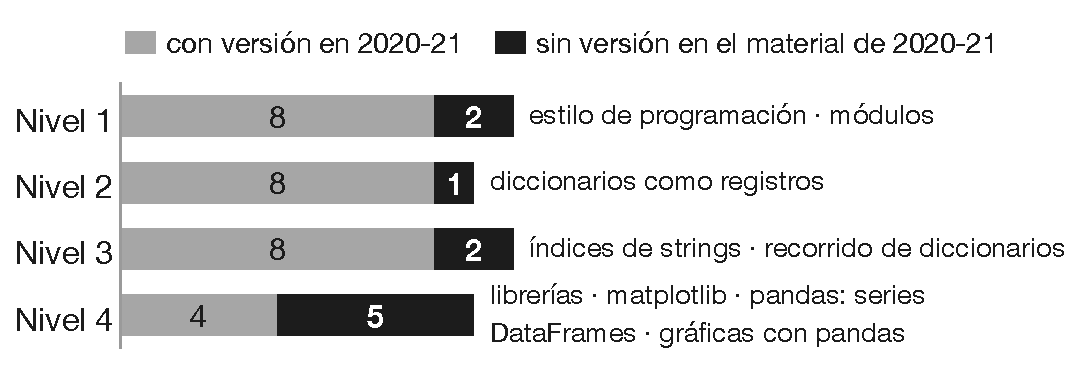
\includegraphics[width=0.92\textwidth]{temas_por_nivel.pdf}
\caption{Clases de 2026-20 por nivel, con y sin versión en el material de 2020-21.}
\label{fig:versiones}
\end{figure}

\textbf{10 de las 38 clases de 2026-20 no tienen versión en el material de 2020-21.} Cinco son del nivel 4: librerías, matplotlib, series y DataFrames de pandas, y gráficas con pandas. En el nivel 1 son estilo de programación y módulos; en el nivel 2, los diccionarios como registros; en el nivel 3, el recorrido de diccionarios y los índices y subcadenas de strings. Dos clases son casos límite. «Más sobre strings» (nivel 3) cuenta sin versión: la clase presenta como nuevos el operador de indexación, las subcadenas y la inmutabilidad, y en el material de 2021-10 el índice y el corte \cod{[:]} solo aparecen para listas; Cadenas solo tiene \cod{find()}. «Separación entre interfaz de usuario y lógica del programa» (nivel 1) cuenta con versión: Funciones (2020-20) ya tiene las secciones «Interfaz básica de un programa», «Input vs Parámetro» y «Print vs Retorno», en las que solo la interfaz lee e imprime; lo que no tenía es llevar la interfaz a otro módulo. «Estructura de datos compuestos» (nivel 3) corresponde a la sección «Estructuras compuestas» de Tuplas, que en 2021-10 era del nivel 4.

La comparación tiene un límite: de 2020-21 hay 12 presentaciones, no el curso completo, así que «sin versión» no prueba que el tema sea nuevo. El programa de 2020-20 ya define el nivel 4 como «solucionar problemas con matrices y librerías»; las librerías probablemente se dictaban con material que no está en el corpus.

{\small\renewcommand{\arraystretch}{1.1}
\begin{longtable}{>{\raggedleft\arraybackslash}p{0.04\textwidth}>{\raggedright\arraybackslash}p{0.46\textwidth}>{\raggedright\arraybackslash}p{0.42\textwidth}}
\caption{Clases de 2026-20 y su versión en el material de 2020-21. Sin introducciones ni ejercicios.}\label{tab:versiones} \\
\toprule
\textbf{N} & \textbf{Clase de 2026-20} & \textbf{Versión en el material de 2020-21} \\
\midrule
\endhead
1 & Descubriendo el mundo de la programación & Análisis y diseño de un programa (2021-10, N1) \\
1 & Valores y tipos de dato & Variables y Expresiones (2020-20, N1) \\
1 & Declaración de variables, instrucción de asignación y tipado dinámico & Variables y Expresiones (2020-20, N1) \\
1 & Expresiones, operadores aritméticos y operaciones sobre strings & Variables y Expresiones (2020-20, N1) \\
1 & Conversion de tipos & Variables y Expresiones (2020-20, N1); Funciones (2020-20, N1) \\
1 & Funciones de Python (Matemáticas y de entrada-salida) & Funciones (2020-20, N1) \\
1 & Funciones y variables locales & Funciones (2020-20, N1) \\
1 & Estilo de programación & \textbf{sin versión} \\
1 & Construcción e importación de módulos & \textbf{sin versión} \\
1 & Separación entre interfaz de usuario y lógica del programa & Funciones (2020-20, N1) \\
2 & Booleanos y sus operadores & Instrucciones Condicionales (2021-10, N2) \\
2 & Tablas de verdad y álgebra booleana & Instrucciones Condicionales (2021-10, N2) \\
2 & Condicionales & Instrucciones Condicionales (2021-10, N2) \\
2 & Leyes de De Morgan & Instrucciones Condicionales (2021-10, N2) \\
2 & Cadenas de caracteres & Cadenas de caracteres (2021-10, N2) \\
2 & Operaciones sobre cadenas de caracteres & Cadenas de caracteres (2021-10, N2) \\
2 & Diccionarios operaciones básicas & Diccionarios (2021-10, N2) \\
2 & Diccionarios mutabilidad, borrado de datos y parámetros por referencia & Diccionarios (2021-10, N2) \\
2 & Diccionarios para manejar elementos con las mismas características & \textbf{sin versión} \\
3 & Instrucciones iterativas (while) & Instrucciones cíclicas (2021-10, N3) \\
3 & Uso del centinela & Instrucciones cíclicas (2021-10, N3) \\
3 & Mas sobre strings & \textbf{sin versión} \\
3 & Instrucciones iterativas (for) & Instrucciones cíclicas (2021-10, N3) \\
3 & Introducción a listas & Listas (2021-10, N3) \\
3 & Operaciones sobre listas & Listas (2021-10, N3) \\
3 & Patrones de recorrido & Patrones de recorrido (2021-10, N3) \\
3 & Recorrido de diccionarios & \textbf{sin versión} \\
3 & Manejo de archivos & Manejo de archivos (2021-10, N3) \\
3 & Estructura de datos compuestos & Tuplas (2021-10, N4); Manejo de archivos (2021-10, N3) \\
4 & Tuplas & Tuplas (2021-10, N4) \\
4 & Estructuras de datos con tuplas & Tuplas (2021-10, N4) \\
4 & Matrices & Matrices (2020-20, N4) \\
4 & Mas sobre matrices & Matrices (2020-20, N4) \\
4 & Introduccion a librerias & \textbf{sin versión} \\
4 & Introduccion a visualizaciones con Matplotlib & \textbf{sin versión} \\
4 & Pandas (series y operaciones sobre series) & \textbf{sin versión} \\
4 & DataFrames & \textbf{sin versión} \\
4 & Visualizacion con pandas & \textbf{sin versión} \\
\bottomrule
\end{longtable}
}

\subsection{Solución híbrida: un agente que contrasta documentos y bodega}
\label{sec:agente}

El filtro de vigencia depende de que alguien etiquete bien cada documento. La bodega ofrece una comprobación independiente: si un documento describe un servicio, los datos dicen si ese servicio opera. El agente (\cod{src/entrega2/agente.py}) hace ese contraste.

\begin{figure}[H]\centering
\begin{tikzpicture}[node distance=0.6cm and 0.9cm]
\node[caja] (q) {Pregunta de la coordinación};
\node[modelo, right=0.6cm of q, text width=3.0cm, minimum height=1.6cm] (ag) {Agente\\gpt-6-luna con llamadas a funciones\\(hasta 8 pasos)};
\node[caja, above right=0.15cm and 0.9cm of ag, text width=3.6cm] (t1) {\cod{buscar\_documentos}\\(consulta, vigencia, semestre)};
\node[caja, right=0.9cm of ag, text width=3.6cm] (t3) {\cod{listar\_presentaciones}\\(semestre, nivel)};
\node[caja, below right=0.15cm and 0.9cm of ag, text width=3.1cm] (t2) {\cod{consultar\_bodega}\\(sql)};
\node[dato, right=0.45cm of t1, text width=3.0cm] (pg) {pgvector, colección visual:\\5 fragmentos con semestre y vigencia};
\node[dato, right=0.45cm of t2, text width=3.0cm] (dw) {Bodega Gold (SQLite):\\vistas de solo lectura};
\node[caja, below=1.0cm of ag, text width=3.4cm] (r) {Respuesta: documento citado, cifras de la bodega y conclusión};
\draw[flecha] (q)--(ag);
\draw[flecha, {Stealth[length=5pt]}-{Stealth[length=5pt]}] (ag.east) -- ++(0.45,0) |- (t1.west);
\draw[flecha, {Stealth[length=5pt]}-{Stealth[length=5pt]}] (ag.east) -- ++(0.45,0) |- (t2.west);
\node[dato, right=0.45cm of t3, text width=3.0cm] (ct) {Catálogo:\\título, semestre y nivel};
\draw[flecha, {Stealth[length=5pt]}-{Stealth[length=5pt]}] (ag.east) -- (t3.west);
\draw[flecha] (t1)--(pg); \draw[flecha] (t3)--(ct); \draw[flecha] (t2)--(dw); \draw[flecha] (ag)--(r);
\end{tikzpicture}
\caption{Flujo del agente. El modelo decide en cada paso qué herramienta usar y con qué argumentos.}
\label{fig:agente}
\end{figure}

\textbf{Herramientas.} \cod{buscar\_documentos} consulta la colección visual y devuelve 5 fragmentos, cada uno con su semestre y su vigencia; el agente decide si incluye versiones anteriores o si busca en un solo semestre. \cod{listar\_presentaciones} devuelve del catálogo los títulos de las presentaciones de un semestre y un nivel, en orden de clase. \cod{consultar\_bodega} ejecuta una sentencia SQL sobre la bodega. La lista del catálogo y el filtro de semestre se agregaron por el caso 8 (sección~\ref{sec:caso8}); los casos 1 a 7 se ejecutaron sin ellos.

\textbf{La bodega que ve el agente} (\cod{src/entrega2/bodega.py}, \cod{sql/e2\_bodega\_vistas.sql}) es una copia del Gold con cuatro vistas y dos tablas agregadas, los tipos de horario y la oferta por semestre. Las vistas resuelven los joins del modelo dimensional y nombran las columnas de forma que el modelo escriba SQL correcto: \cod{v\_reservas} (una fila por reserva, con período, semana, tipo de tutoría y estado), \cod{v\_encuestas}, \cod{v\_respuestas} y \cod{v\_oferta\_franja} (capacidad, ocupación y lista de espera de cada franja). Su descripción va en las instrucciones del agente. Tres controles limitan lo que puede hacer: la conexión es de solo lectura; se admite una sola sentencia \cod{SELECT}, de hasta 200 filas y con un límite de trabajo; y la copia no contiene los 25.256 comentarios de texto libre de las encuestas ni permite leer \cod{dim\_programa}, donde la fuente trae nombres de personas.

\textbf{Instrucciones.} El agente debe buscar la regla en los documentos, identificar la versión vigente, comprobarla con una consulta agregada, comparar versiones listando el nivel en cada semestre y buscando en el semestre viejo los temas que difieren, no afirmar nada que no venga de una herramienta y cerrar con tres partes: qué dice el documento, qué muestra la bodega y si coinciden.

\subsection{Resultados del agente}

Ocho casos (\cod{data/bronce/evaluacion/preguntas\_agente.json}) prueban el agente; sus trazas completas están en \cod{artifacts/entrega2/resultados/agente/casos.json}.

\begin{table}[H]\small\renewcommand{\arraystretch}{1.15}
\begin{tabularx}{\textwidth}{L>{\raggedright\arraybackslash}p{0.24\textwidth}RRR}
\toprule
\textbf{Caso} & \textbf{Herramientas usadas} & \textbf{Pasos} & \textbf{Tiempo (s)} & \textbf{USD} \\
\midrule
¿Se siguen ofreciendo las tutorías grupales del programa? & documentos, bodega & 2 & 4,9 & 0,0004 \\
Qué no deben hacer los tutores y a qué se dedica la tutoría & documentos, bodega (3) & 4 & 7,5 & 0,0006 \\
Semanas de mayor demanda frente al cierre de los niveles & documentos, bodega (3) & 4 & 9,0 & 0,0009 \\
Uso de IA por los tutores según las encuestas & documentos (2), bodega (4) & 6 & 11,4 & 0,0011 \\
Reservas e inasistencia por semestre desde 2023 & bodega & 1 & 4,5 & 0,0003 \\
Cómo explica el curso el recorrido parcial con centinela & documentos & 1 & 3,5 & 0,0003 \\
¿Se ajustó la oferta de cupos a la caída de las reservas? & documentos, bodega (7) & 8 & 15,5 & 0,0017 \\
Qué se dicta hoy en el nivel 3 que no está en el material de 2021-10 & catálogo (2), documentos (2) & 4 & 7,3 & 0,0007 \\
\bottomrule
\end{tabularx}
\end{table}

El agente eligió bien las herramientas: usó solo la bodega en la pregunta numérica, solo documentos en las dos de contenido (en el caso 8, también el catálogo) y documentos y bodega en las cuatro híbridas. En la pregunta de oferta buscó primero una regla de cupos en los documentos; no la hay, y lo dijo. Ninguna consulta SQL falló por sintaxis.

\textbf{Caso 1, la salida que pide el enunciado.} Pregunta: «El programa del curso menciona tutorías grupales en CupiTaller. ¿Se siguen ofreciendo?». El agente buscó en todas las versiones, ejecutó \cod{SELECT periodo, tipo\_horario, SUM(reservas) FROM agg\_tipos\_de\_horario WHERE tipo\_horario LIKE '\%Grupal\%' GROUP BY periodo, tipo\_horario} y respondió:

\begin{quote}\small
El programa vigente que aparece en la búsqueda no especifica si hay tutorías grupales; la mención explícita encontrada dice que existen tutorías individuales, grupales y express, pero corresponde a [Programa del curso IP, semestre 2020-20, p. 5], \textbf{no vigente}. [...] La bodega muestra registros de «Deprecated, Grupal» hasta el período \textbf{202120} (118 reservas) y de «Deprecated, Express grupal» en \textbf{201910} (157). No aparecen registros de tipos grupales después de 202120 en \cod{agg\_tipos\_de\_horario}. \textbf{Conclusión:} la evidencia disponible no indica que las tutorías grupales se sigan ofreciendo; la última actividad registrada bajo esos tipos fue en 2021-20.
\end{quote}

Las cifras coinciden con la bodega: 777 reservas grupales entre 2017-10 y 2021-20, y ninguna después.

\textbf{Caso 2, regla frente a uso.} El agente citó la regla vigente (los tutores no solucionan proyectos) y encontró que «Resolver un problema en mi proyecto» es la respuesta más frecuente sobre el uso de la tutoría: 10.236 de 19.672 (52\,\%). Concluyó que hay una tensión, y que la encuesta no dice quién resolvió el problema, de modo que no prueba un incumplimiento. Es la lectura correcta de un dato de encuesta.

\textbf{Caso 3, demanda y niveles.} El agente derivó del programa que los niveles, de 9, 12, 15 y 12 sesiones a tres por semana, cierran cerca de las semanas 3, 7, 12 y 16, y comparó con las reservas por semana. Reportó una coincidencia parcial y advirtió que la semana de la bodega es aproximada. La figura~\ref{fig:demanda} muestra el patrón completo: cuatro olas por semestre, cada una con una caída después del pico (en 2024-20, de 356 a 56 reservas, de 622 a 128, de 443 a 67 y de 589 a 201). El programa explica la forma: cada nivel termina con un proyecto y un examen basado en él, y el proyecto es el uso principal de la tutoría.

\begin{figure}[H]\centering
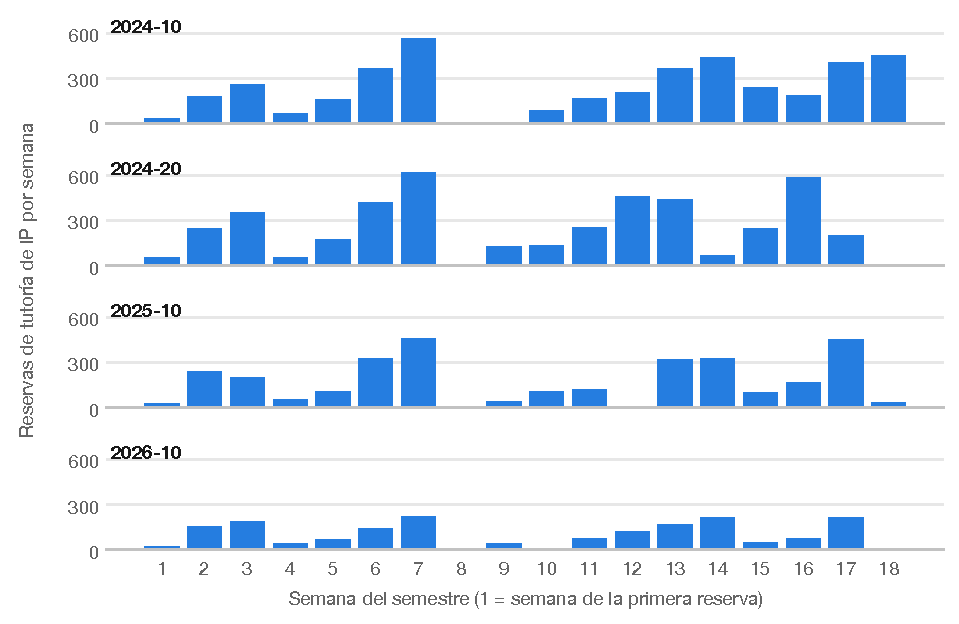
\includegraphics[width=0.9\textwidth]{demanda_semanal.pdf}
\caption{Reservas de tutoría de IP por semana en cuatro semestres. Las semanas sin barra no tienen reservas (recesos).}
\label{fig:demanda}
\end{figure}

\textbf{Caso 4, IA en las tutorías.} El agente distinguió el alcance de la regla: el programa prohíbe el contenido de chatbots en los entregables del estudiante y no regula el uso de IA por el tutor. En las encuestas, 362 respuestas dicen que el tutor usó una herramienta de IA y 8.321 que no. No concluyó un incumplimiento. Para la coordinación, el hallazgo es que falta una regla escrita para ese caso.

\textbf{Caso 5, oferta frente a demanda.} Con \cod{agg\_oferta\_periodo}, el agente encontró que la capacidad pasó de 2.703 cupos en 2024-20 a 2.797 en 2025-10 y a 2.616 en 2025-20 y 2026-10, mientras la ocupación bajó de 81,2 a 54,1 y 55,0\,\%. Con \cod{v\_oferta\_franja} ubicó la lista de espera de cada semestre junto con la capacidad de esa franja: martes a las 8:00 en 2025-10 (17 solicitudes, 26 de 29 cupos reservados), miércoles a las 14:00 en 2025-20 (11 solicitudes, 46 de 60) y en 2026-10 (8 solicitudes, 44 de 55). Concluyó que la capacidad bajó menos que las reservas y que ningún documento fija una regla de cupos con la cual contrastarlo. La capacidad es del semestre completo, así que una franja puede tener cupos libres en el total y lista de espera en semanas puntuales: el viernes a las 12:30 de 2026-10 tuvo 26 de 50 cupos reservados y 4 solicitudes en lista. Las cifras coinciden con la bodega.

\textbf{Caso 8, qué cambió en el nivel 3.}\label{sec:caso8} Pregunta: «Soy profesor del nivel 3 de IP y tengo las presentaciones de 2021-10. ¿Qué temas se dictan hoy en el nivel 3 que no aparecen en ese material?». Es una pregunta de inventario, y la búsqueda por similitud no la resuelve sola: cada búsqueda trae 5 fragmentos sueltos. El agente respondió al cuarto intento. La traza final está en \cod{artifacts/entrega2/resultados/agente/casos.json} y las tres anteriores en \cod{docs/entregables/e2\_informe/ag-08\_intentos\_previos.json}; esas no se pueden reproducir con el código actual, que ya tiene los tres cambios.

\begin{enumerate}[leftmargin=1.8em,itemsep=2pt]
\item Con las dos herramientas originales hizo 8 búsquedas y agotó los pasos sin responder.
\item Con \cod{listar\_presentaciones} listó solo el nivel 3 de 2021-10 y concluyó que no podía comparar.
\item Con una instrucción para comparar versiones (listar el nivel en cada semestre y comprobar con búsquedas los temas que solo aparezcan en la lista nueva) listó los dos semestres, pero volvió a agotar los pasos: la búsqueda solo distinguía vigente de no vigente, y sobre todo el corpus las 44 presentaciones vigentes tapan a las 12 viejas.
\item Con un filtro de semestre en \cod{buscar\_documentos} respondió en 4 pasos, 7,3 s y US\$ 0,0007: listó las 4 presentaciones de 2021-10 y las 12 de 2026-20, y buscó solo en 2021-10 los temas que difieren.
\end{enumerate}

\begin{quote}\small
El material vigente de nivel 3 incluye \textbf{Recorrido de diccionarios} como tema explícito [\emph{Recorrido de diccionarios}, 2026-20, p. no indicada; vigente]. [\ldots] el material disponible de 2021-10 sí trata diccionarios en nivel 2 [\ldots]. Por eso, \textbf{el tema que destaca como nuevo en la secuencia actual de nivel 3 es el recorrido de diccionarios}; no puedo concluir que los diccionarios no aparecieran en el curso anterior. La comparación es limitada: no tenemos aquí el curso completo de 2021-10, y las listas de presentaciones solo indican títulos, no todo el contenido.
\end{quote}

La respuesta acierta una de las dos clases del nivel 3 sin versión en la tabla~\ref{tab:versiones}, el recorrido de diccionarios, y omite la otra: «Más sobre strings». Al buscar strings en 2021-10 recuperó páginas de Diccionarios, Instrucciones cíclicas y Listas, no la de Cadenas, y no volvió a la clase. No tomó por nuevas «Uso del centinela» ni «Estructura de datos compuestos», que tienen títulos nuevos pero contenido que ya estaba en 2021-10. Llama «nuevo» al tema, una palabra que este informe evita porque el material de 2021-10 está incompleto; el propio agente lo advierte en la misma respuesta. Tiene dos defectos de cita: atribuye la lista de títulos a «[Diccionarios, 2021-10, p. 2]», cuando vino del catálogo, y no indica la página de la clase vigente. El agente se ajustó sobre este mismo caso, así que su resultado sobreestima el desempeño en preguntas parecidas; repetir la pregunta para los niveles 1, 2 y 4 es la prueba que falta.

\subsection{Limitaciones}

\begin{itemize}[leftmargin=1.5em,itemsep=2pt]
\item La semana del período se cuenta desde la primera reserva, porque Bookeau no guarda el calendario académico. El desfase con la semana de clases es de una o dos semanas. Indexar el cronograma de cada semestre lo resolvería.
\item Las etiquetas de semestre de los documentos históricos se infieren de la fecha del archivo. \pendiente{confirmar con quien entregó las presentaciones que C3, C4 y Matrices son de 2020-20 y el resto de 2021-10}
\item Los ocho casos del agente son una demostración, no una medición de exactitud. Cada caso se revisó contra la bodega o, el caso 8, contra la correspondencia de la tabla~\ref{tab:versiones}.
\item El agente depende de un modelo externo. Lo que lee, páginas del curso y resultados agregados, sale de la Universidad; por eso la copia de la bodega no tiene texto libre ni nombres.
\end{itemize}

\section{Fase 5 · Gestión del proyecto}

\subsection{Contribuciones y distribución de puntos}

\begin{table}[H]\small\renewcommand{\arraystretch}{1.15}
\begin{tabularx}{\textwidth}{>{\raggedright\arraybackslash}p{0.2\textwidth}LRL}
\toprule
\textbf{Integrante} & \textbf{Trabajo realizado} & \textbf{Puntos} & \textbf{Justificación} \\
\midrule
María Alejandra Pérez Petro & \pendiente{trabajo realizado} & \pendiente{puntos} & \pendiente{justificación} \\
Santiago Martinez Novoa & \pendiente{trabajo realizado} & \pendiente{puntos} & \pendiente{justificación} \\
\bottomrule
\end{tabularx}
\end{table}

\pendiente{criterios de la guía (compromiso, calidad, cumplimiento, participación), problemas del equipo y estrategias. La Entrega 1 fijó como estrategia pedir a la coordinación las definiciones en la primera semana y automatizar el flujo de punta a punta; conviene decir si se cumplió}

\subsection{Uso de herramientas de IA generativa}

\textbf{Declaración del uso.}

\begin{table}[H]\small\renewcommand{\arraystretch}{1.15}
\begin{tabularx}{\textwidth}{>{\raggedright\arraybackslash}p{0.26\textwidth}L}
\toprule
\textbf{Herramienta} & \textbf{Tipo de uso} \\
\midrule
Claude Code (asistente de programación de Anthropic) & Revisión del enunciado, de la Entrega 1 y del corpus; propuesta de los requerimientos y de la arquitectura; generación del código de ingesta, RAG, prompting directo, agente, evaluación y gráficas; ejecución de las corridas; depuración; redacción del borrador de este informe y del póster. \\
\cod{gpt-6-luna} (OpenAI) & Componente del sistema: transcribe las páginas, responde en los dos enfoques y es el modelo del agente. \\
\cod{gpt-6-sol} (OpenAI) & Componente de la evaluación: juez de las respuestas. \\
\bottomrule
\end{tabularx}
\end{table}

\textbf{Prompts utilizados.} Los prompts al asistente de programación fueron cuatro, en una sola sesión:

\begin{enumerate}[leftmargin=1.5em,itemsep=2pt]
\item «Revisa los documentos que te puse aquí, así como el proyecto 1 para el contexto. La idea es que me ayudes a plantear todo el nuevo sistema y todo este proyecto de manera clara.»
\item «Yo tengo las del semestre del 2021. Lo otro es que seguramente nos tocará hacer un RAG visual, ¿no? [...] Todo lo viejo quedó en \emph{data antigua} para que se pueda etiquetar adecuadamente.»
\item «Hacemos absolutamente todo. Es para el jueves.»
\item «Igual piensa que tenemos API de Anthropic, también podemos usar esa.»
\end{enumerate}

Los prompts del sistema están en el código y se pueden leer completos: las instrucciones de transcripción (\cod{src/entrega2/transcribir.py}), las reglas de respuesta (\cod{src/entrega2/enfoques.py}), las instrucciones del agente (\cod{src/entrega2/agente.py}) y las del juez (\cod{src/entrega2/juez.py}).

\textbf{Análisis crítico del resultado.} Estos son los puntos en que la primera propuesta o la primera versión de la IA se cambió, y por qué. \pendiente{cada integrante debe revisar esta lista, corregirla y añadir su propio análisis: qué conceptos del curso le permitieron evaluar la respuesta}

\begin{itemize}[leftmargin=1.5em,itemsep=2pt]
\item \textbf{Alcance.} La IA propuso primero decidir si recortar el bono y la ingesta visual según el tiempo disponible. El equipo decidió hacer todas las fases, incluido el agente.
\item \textbf{Corpus.} La IA señaló que con una sola versión de los documentos no había un caso real de inconsistencia. El equipo consiguió el programa de 2020-20 y las presentaciones de 2020 y 2021, y propuso la ingesta visual.
\item \textbf{Bodega.} El Gold que había en disco era anterior a las reglas R03, R06 y R07 (86.562 reservas). Se reconstruyó con el código final de la Entrega 1 hasta obtener las 83.894 reservas del informe anterior.
\item \textbf{Costo del prompting directo.} La primera medición no leía la caché del proveedor y no contaba el recargo por escribirla. Se corrigió con un punto de corte explícito y el costo por consulta bajó de US\$\,0,0103 a 0,0011.
\item \textbf{Banco de preguntas.} Cuatro respuestas esperadas pedían más de lo que preguntaba la pregunta y producían veredictos «parcial» injustos. Se ajustaron y se repitió toda la evaluación.
\item \textbf{Privacidad.} La IA retiró de la copia de la bodega los comentarios de texto libre y las portadas con nombre y correo, de acuerdo con el riesgo de privacidad que el equipo documentó en la Entrega 1.
\end{itemize}

\textbf{Aportes propios.} \pendiente{cada integrante: qué desarrolló, modificó o decidió; qué ajustó sobre el código o la explicación de la IA; qué aprendió. Hechos verificables en la sesión: el equipo eligió el dominio y el corpus, consiguió los documentos históricos, pidió etiquetarlos por versión, planteó el RAG visual y decidió el alcance}

\appendix
\section{Cómo reproducir}

\begin{verbatim}
brew install postgresql@18 pgvector
python3 -m venv .venv && source .venv/bin/activate
pip install -r requirements.txt
scripts/e2_postgres.sh iniciar
python3 src/main.py               # Entrega 1 (datos reales): Silver y Gold en data/
python3 src/main.py --entrega 2   # catálogo, transcripción, índice, bodega,
                                  # evaluación, prueba de concepto, agente y figuras
python3 src/entrega2/agente.py "¿Se siguen ofreciendo las tutorías grupales?"
\end{verbatim}

El \cod{README.md} describe cada paso, los datos que no se versionan y las decisiones de diseño.

\end{document}
